\documentclass{article}
\usepackage[margin=0.80in, a4paper]{geometry} % Adjust margins here
\usepackage{amsmath}
\usepackage{booktabs} % For better looking tables
\usepackage{float}
\usepackage{url} % For formatting URLs
\usepackage{hyperref}
\usepackage{subcaption}
\usepackage{graphicx} % subcaption for subfigure environment
\graphicspath{{./img/}}
%%%%%%%%%%%%%%%%%%%%%%%%%%%%%%%%%%%%%%%%%%%%%%%%%%%%%%%%%%%%%%%%%
\author{Francesco Sermi\\Francesco Angelo Fabiano Antonacci}

\date{\today}
\title{Relazione FFT}
%%%%%%%%%%%%%%%%%%%%%%%%%%%%%%%%%%%%%%%%%%%%%%%%%%%%%%%%%%%%%%%%%

\begin{document}
\maketitle

\section{Forme d'onda}
    
        E' stata fatta la FFT di forme d'onda quadrate, trinagolari e sinusoidali
        acquisite in laboratorio
        Il risultato è mostrato in Fig.($\ref{fig:for_ond}$).

    \begin{figure}[H]
        \centering
        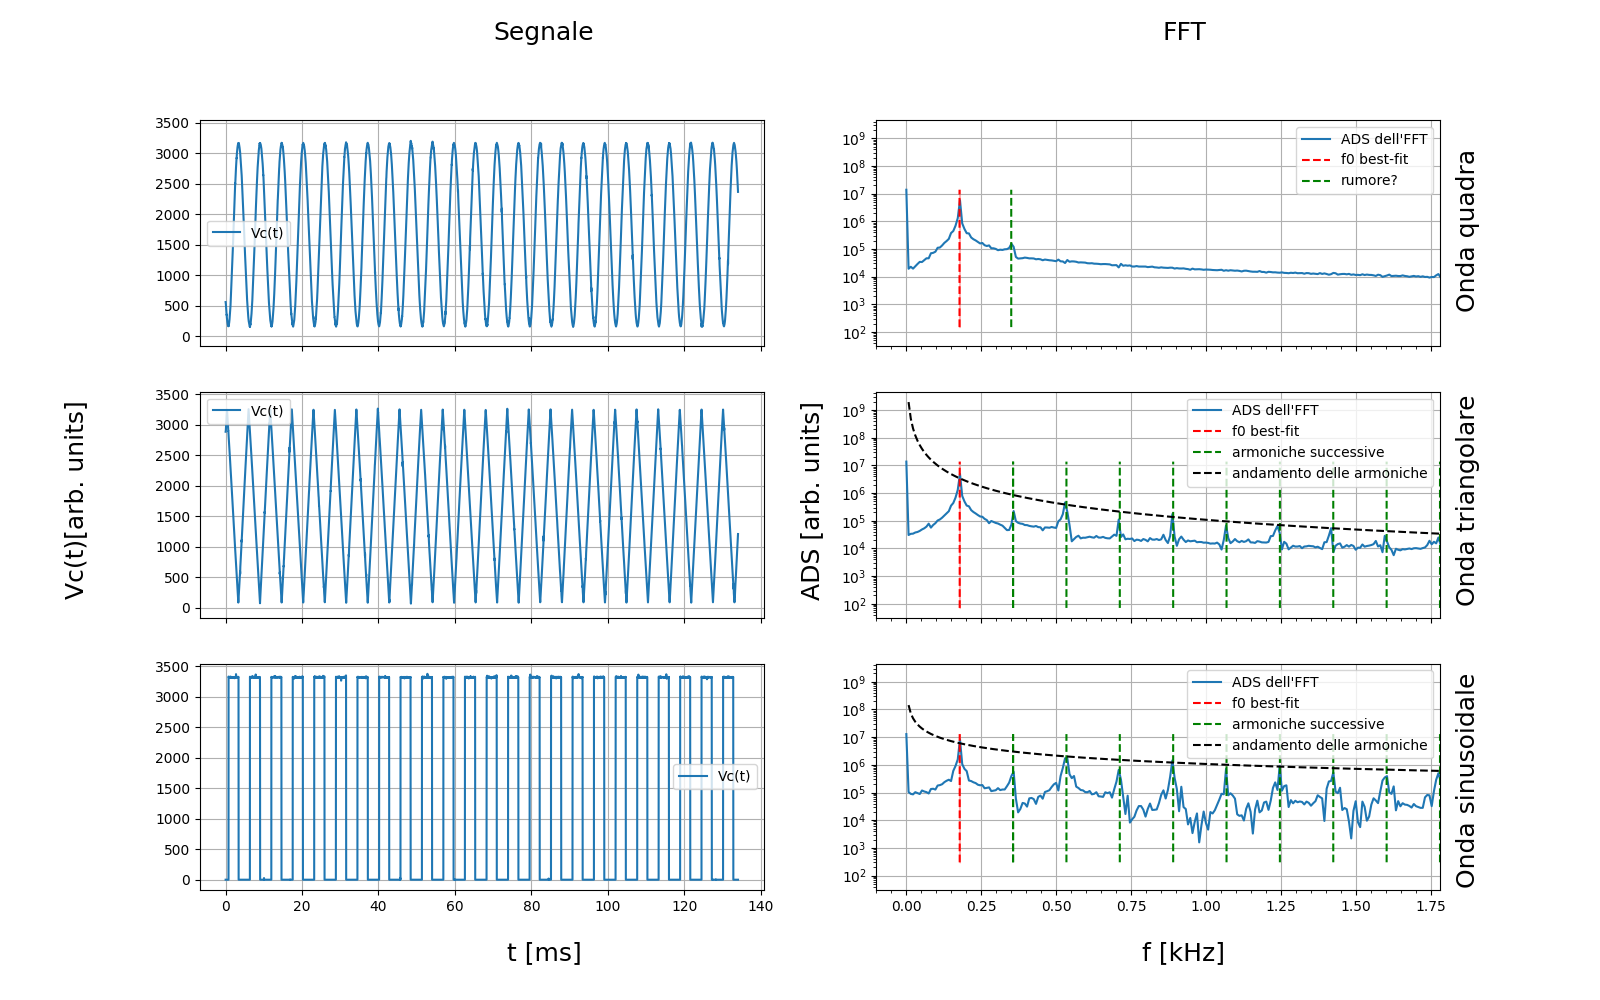
\includegraphics[width=\textwidth]{FFT5/FFTwaveforms1.png}
        \caption{A destra sono mostrati segnali acquisiti in laboratorio, a sinistra 
                è stata eseguita la FFT.}
        \label{fig:for_ond}
    \end{figure}    

        Nel caso dell'onda sinusoidale si osseva la comparsa di un picco dovuto a 
        rumore a $300$[Hz].
        Per le altre forme d'onda è interessante notare la comparsa delle 
        armoniche successive alla principale, come ci si aspetta dallo 
        sviluppo in serie di seni e coseni delle rispettive forme d'onda.
        In questi casi è stata diseganta sopra la FFT
        la legge di potenza di come scalano le armoniche successive , rispettivamente
        $\frac{1}{k}$ e $\frac{1}{k^2}$ per l'onda quadra e  per quella triangolare.

        E' stato eseguito un bestfit per le frequenze principali $f_0$, i risultati 
        sono riportati in Tab.($\ref{tab:for_ond}$) e 
        mostrati in Fig.($\ref{fig:for_ond}$) assieme al rispettivo valore 
        estrapolato dalla FFT.

        Come incertezza sulla frequenza $f_0$ estrapolata dalla FFt è stata 
        considerata la deviazione standard di una distribuzione uniforme attorno
        a $f_0$ con ampiezza la risoluzione del campionamento:si assume infatti
         che ogni punti attorno a $f_0$ possa essere equiprobabilmente il "valore reale".  
         

        \begin{table}[H]
            \centering
            \caption{Confronto tra le frequenze di oscillazione misurate con quelle ottenute tramite FFT e bestfit.
                    Attorno ai valori medi è stata rappresentata la barra di errore per il valore
                    misurato e per quello del bestfit, per il quale non si vede essendo molto piccola.}
                \begin{tabular}{ccc}
                    onda            &   $f_{0fft}$[kHz]                     & $f_{0bestfit}$[kHz] \\
                    \hline
                    Sinusoide       &   $0.179 \pm 0.001$           & $0.177455 \pm 0.000002$ \\
                    Triangolare     &   $0.179 \pm 0.001$           & $0.1780571\pm 0.0000009$ \\
                    Quadra          &   $0.179 \pm 0.001$           & $0.1780571 \pm 0.0000009$ \\
                \end{tabular}
                \caption{I tre segnali sono stati raccolti a distanza di poco tempo
                        cambiando solo la forma d'onda con il generatore di funzioni,
                        tuttavia colpisce la vicinanza dei valori $f_{0fft}$.
                        Nessuno dei valori per la frequenza acqusito con la FFT
                        e col Fit sono compatibili nella barra di errore.
                        Potrebbe essere stato sottostimato l'errore nella FFT.}
                \label{tab:for_ond}
        \end{table}

        Sono state anche fatte acquisizioni "lunghe" di forme d'onda sinusoidali
         e quadrate. Sono riportati i risultati del bestfit in Fig.($\ref{fig:for_lun}$)
         e in Tab.($\ref{tab:for_lun}$)

         

         \begin{figure}[H]
            \centering
            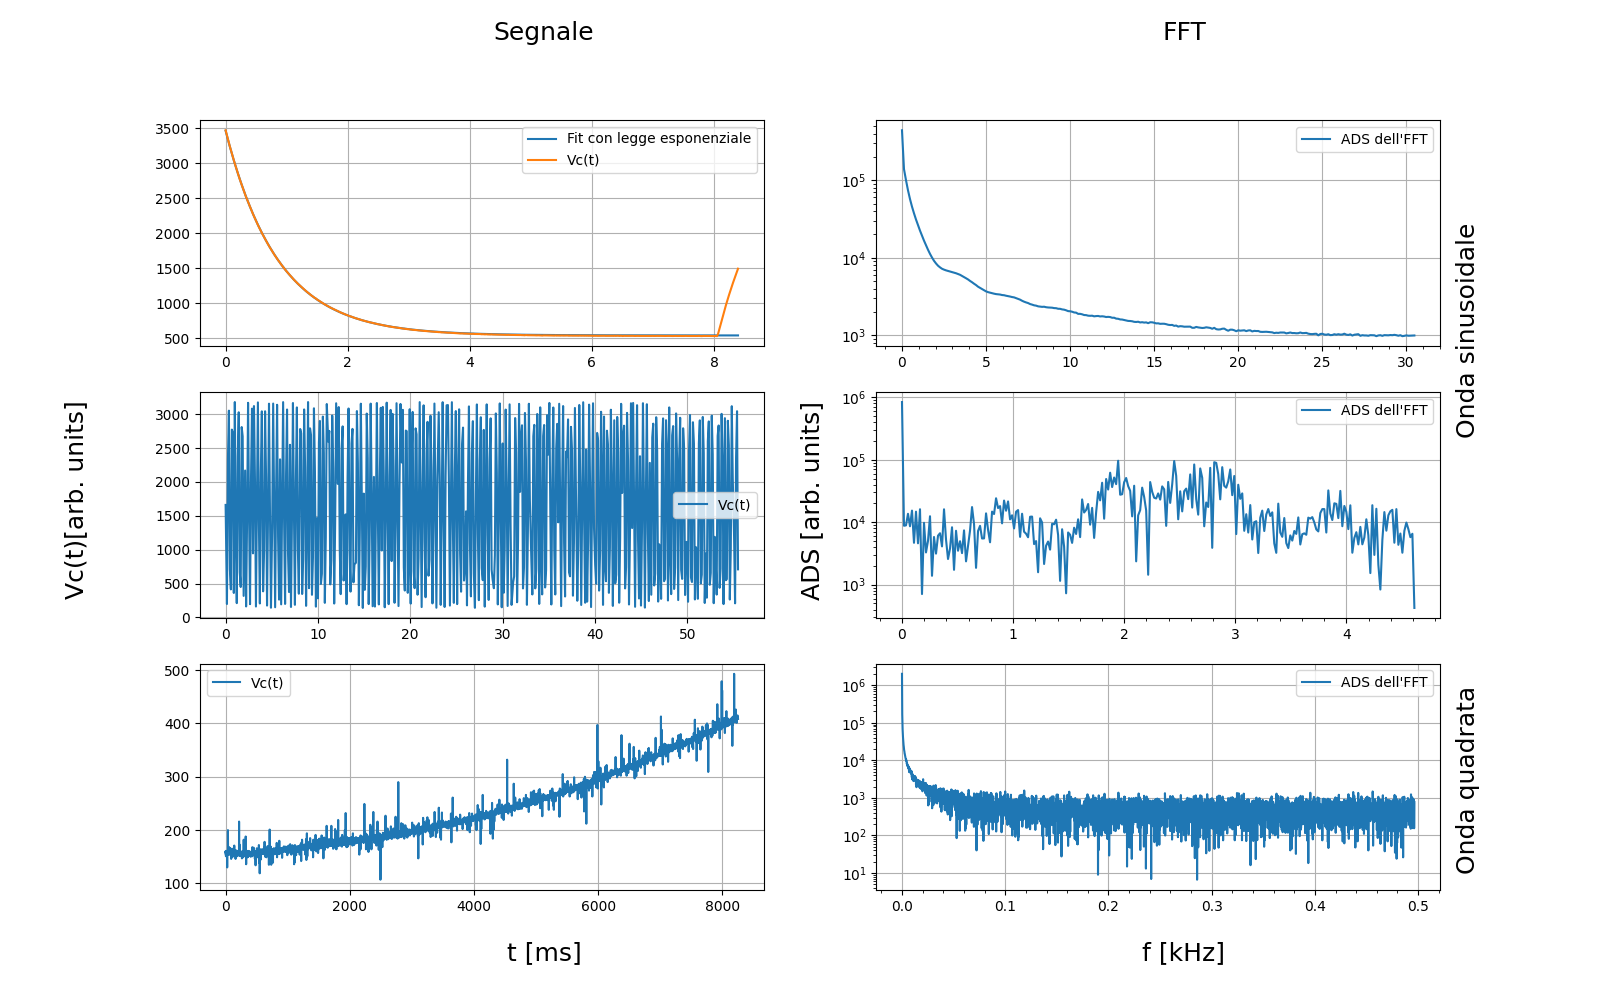
\includegraphics[width=\textwidth]{FFT5/FFTwaveforms3.png}
            \caption{A destra sono mostrati segnali acquisiti in laboratorio, a sinistra 
                    è stata eseguita la FFT.
                    E' molto interessante osservare che nel caso dell'onda quadra 
                    non compare l'armonica successiva aspettata: questo potrebbe essere 
                    legato al fatto che in media sono presi sette punti per periodo e quindi 
                    è possibile che ci sia un sottocampionamento dei dati per questa analisi.}
            \label{fig:for_lun}
        \end{figure}    


         \begin{table}[H]
            \centering
            \caption{}
                \begin{tabular}{ccc}
                    onda            &   $f_{0fft}$[kHz]                     & $f_{0bestfit}$[kHz] \\
                    \hline
                    Sinusoide       &   $0.13354 \pm 0.00002$           & $0.13352992 \pm 0.0000003$ \\
                    Quadra          &   $0.13354 \pm 0.00002$           & $0.1334881 \pm  0.000003$ \\
                \end{tabular}
                \caption{Similmente a quanto accade in Tab.($\ref{tab:for_ond}$) le 
                frequenze estrapolate con FFT sono molto vicine tra loro e molto precise;
                le frequenze estrapolate con FFT e bestfit sono molto vicine tuttavia non 
                sono compatibili dentro la barra di errore.}
                \label{tab:for_lun}
        \end{table}
        


\section{Forme d'onda distorte}

        Sono stati raccolti segnali cambiando il duty cycle ed è stato eseguito un fit 
        con una sinusoide con l'obbiettivo di far convergere solo la frequenza.

        E' stata realizzata per ciascuna forma d'onda l'FFT.
        Il risultato della manipolazione dei dati è riporato in Fig.($\ref{fig:for_dis}$)
        e in Tab.($\ref{tab:for_dis}$).
        \begin{figure}[H]
                \centering
                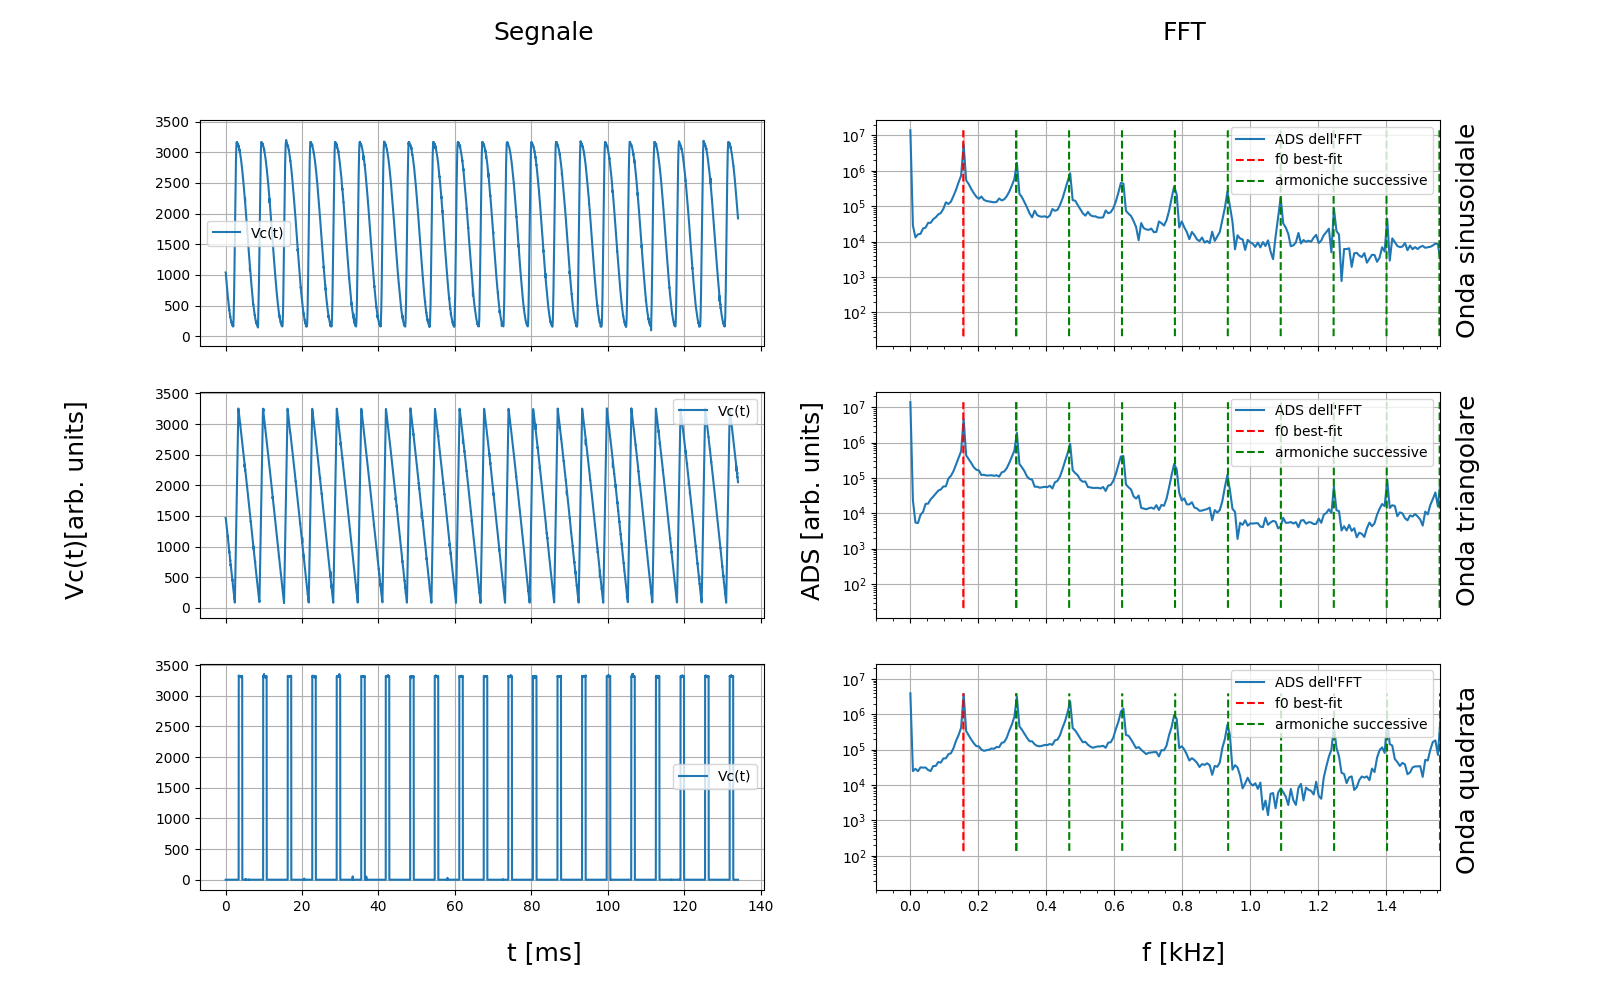
\includegraphics[width=\textwidth]{FFT5/FFTwaveforms2.png}
                \caption{A destra sono mostrati segnali acquisiti in laboratorio, 
                        a sinistra è stata eseguita la FFT.
                        Attorno ai valori medi è stata rappresentata la barra di 
                        errore per il valore misurato e per quello del bestfit, 
                        per il quale non si vede essendo molto piccola.}
                \label{fig:for_dis}
        \end{figure}   

        \begin{table}[H]
            \centering

                \begin{tabular}{ccc}
                    onda            &   $f_{0fft}$[kHz]                     & $f_{0bestfit}$[kHz] \\
                    \hline
                    Sinusoide       &   $0.156 \pm 0.001$           & $0.15559 \pm 0.00002$ \\
                    Triangolare     &   $0.156 \pm 0.001$           & $0.15559 \pm 0.00002$ \\
                    Quadra          &   $0.156 \pm 0.001$           & $0.15576 \pm 0.00006$ \\
                \end{tabular}
                \caption{I tre segnali sono stati raccolti a distanza di poco tempo
                cambiando solo la forma d'onda con il generatore di funzioni,
                tuttavia colpisce la vicinanza dei valori $f_{0fft}$.
                Nessuno dei valori per la frequenza acqusito con la FFT
                e col Fit sono compatibili nella barra di errore.
                Potrebbe essere stato sottostimato l'errore nella FFT.}
                \label{tab:for_dis}
        \end{table}

\section{Cattive acquisizioni}

    In Fig.($\ref{fig:merda}$) sono riportati esempi di "cattive acquisizioni".

        \begin{figure}[H]
            \centering
            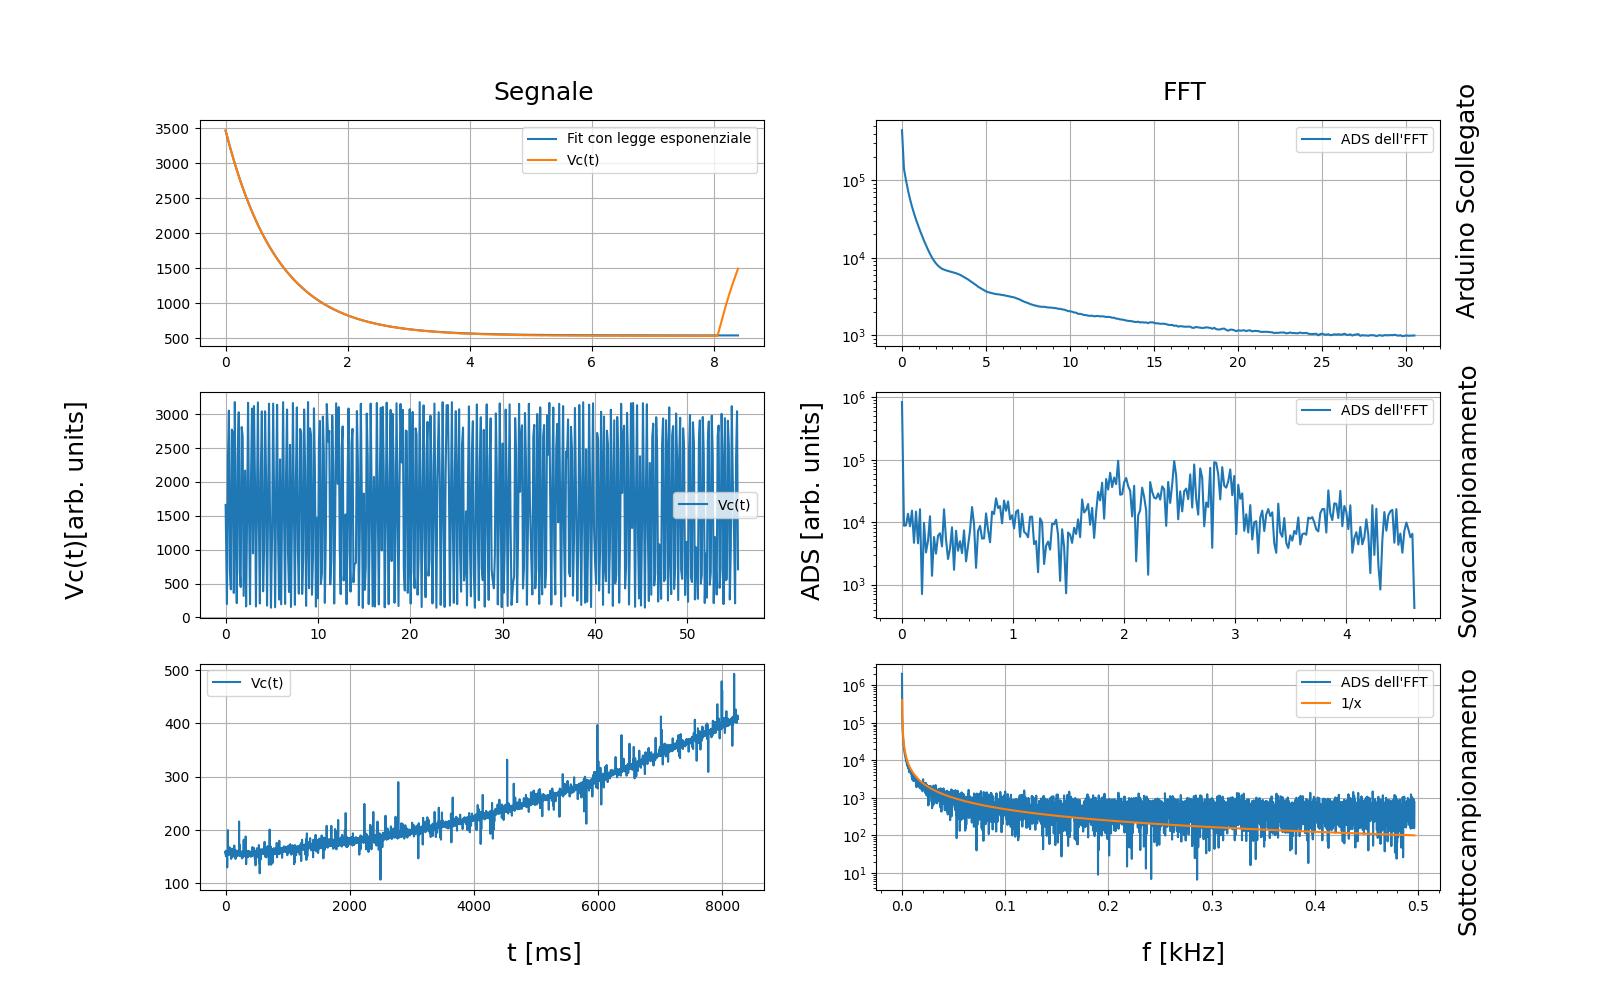
\includegraphics[width=\textwidth]{FFT5/FFTwaveforms4.png}
            \caption{I primi due grafici rappresentano il campionamento di una porta di arduino scollegata.
            In mezzo è riporato un sottocampionamento: per ogni periodo è acquisito un 
            solo punto.
            La terza coppia di figure dall'alto rappresenta un sovracampionamento 
            di un periodo: l'acquizione prende  solo il ramo crescente di un seno.}
            \label{fig:merda}
        \end{figure}  
    
    E' stato eseguito un bestfit con una legge esponenziale per la sezione decrescente
    del segnale acquisito con arduino scollegato: fisicamente questo è legato all'ipotesi 
    che una certa carica presente prima dell'acquisizione 
    sulla porta è dissipata quando la porta comunica con il resto di Arduino.
    Il risultato del bestfit è riporatto in Tab.($\ref{tab:merda}$)

        \begin{table}[H]
            \centering
            \begin{tabular}{cc}
                $\tau[ms]$ & $\chi^2_{norm}$\\
                \hline
                $0.8598\pm0.0004$ &$5$\\
            \end{tabular}
        \caption{Risultati bestfit per legge esponenziale di un'acquisizione 
                con arduino scollegato. $\tau$ è il tempo di decadimento della legge 
                esponenziale.}
        \label{tab:merda}
        \end{table}



    Per quanto riguarda il sovracampionamento è sufficiente dire che la 
    FFT non riesce a trovare l'armonica principale del segnale sinusoidale e 
    che i diversi picchi che compaiono nel segnale possono esseredi natura puramente
    accidentale.

    Nel caso di sottocampionamento siccome una sinusoide localmente può 
    essere approssimata con una retta, si è disegnato sopra la FFT la funzione
    $\frac{\alpha}{f}$ -dove $\alpha$ è una costante arbitraria-
    in quanto ciascun termine dello sviluppo in serie  di 
    armoniche della funzione $g(f)=f$ è proporzionale all'inverso della 
    corrispettiva frequenza.







\section{Autoscillatore}

    Sono state prese delle misure di un segnale in uscita da un autoscillatore, il cui schema è riportato in Fig(\ref{fig:circuitino_oscillante})
        \begin{figure}[H]
            \centering
            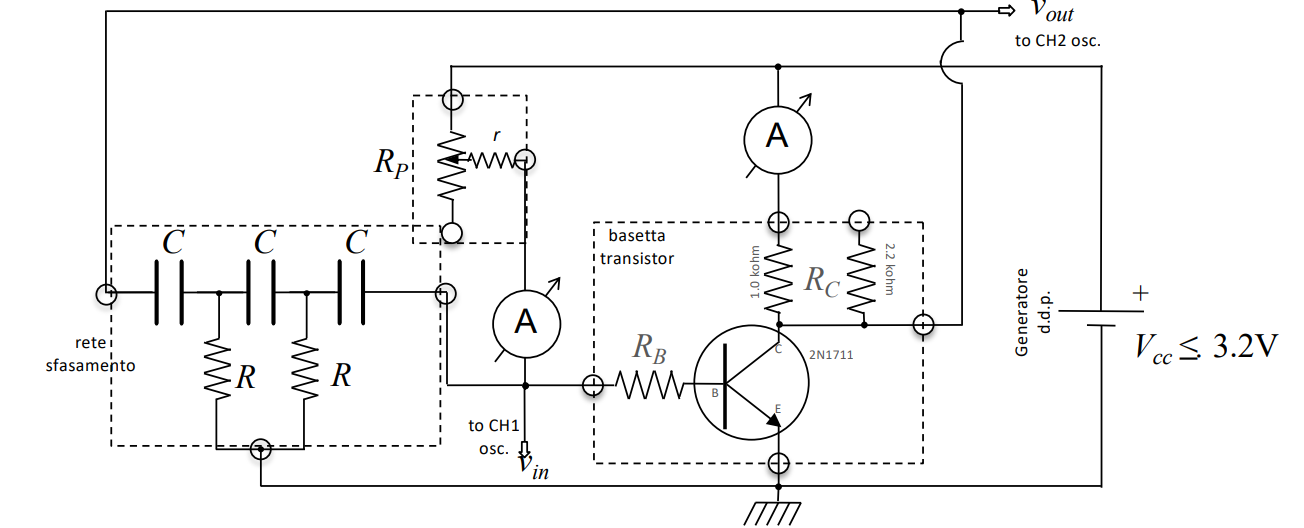
\includegraphics[scale=0.30]{FFT11/schema_circuitino.png}
            \caption{Schema circuitale dell'oscillatore}
            \label{fig:circuitino_oscillante}
        \end{figure}

    Per ogni segnale registrato, è stato eseguito il fit ai minimi quadratici per individuare la frequenza dell'oscillazione sinusoidale del segnale in uscita, usando la seguente funzione modello
        $$
            f(t; A, \omega, \phi, c) = A \sin{(\omega t + \phi)} + c,
        $$
    confrontandolo con il contenuto spettrale ottenuto tramite l'algoritmo della RFFT.
    Riportiamo in Fig(\ref{fig:sign_rfft_autoscill}) i grafici con a sinistra il segnale in uscita e a destra la trasformata di Fourier del segnale, dove viene graficato una linea verticale che rappresenta il valore stimato di $f = \frac{\omega}{2 \pi}$ stimato dal bestfit
        \begin{figure}[H]
            \centering
            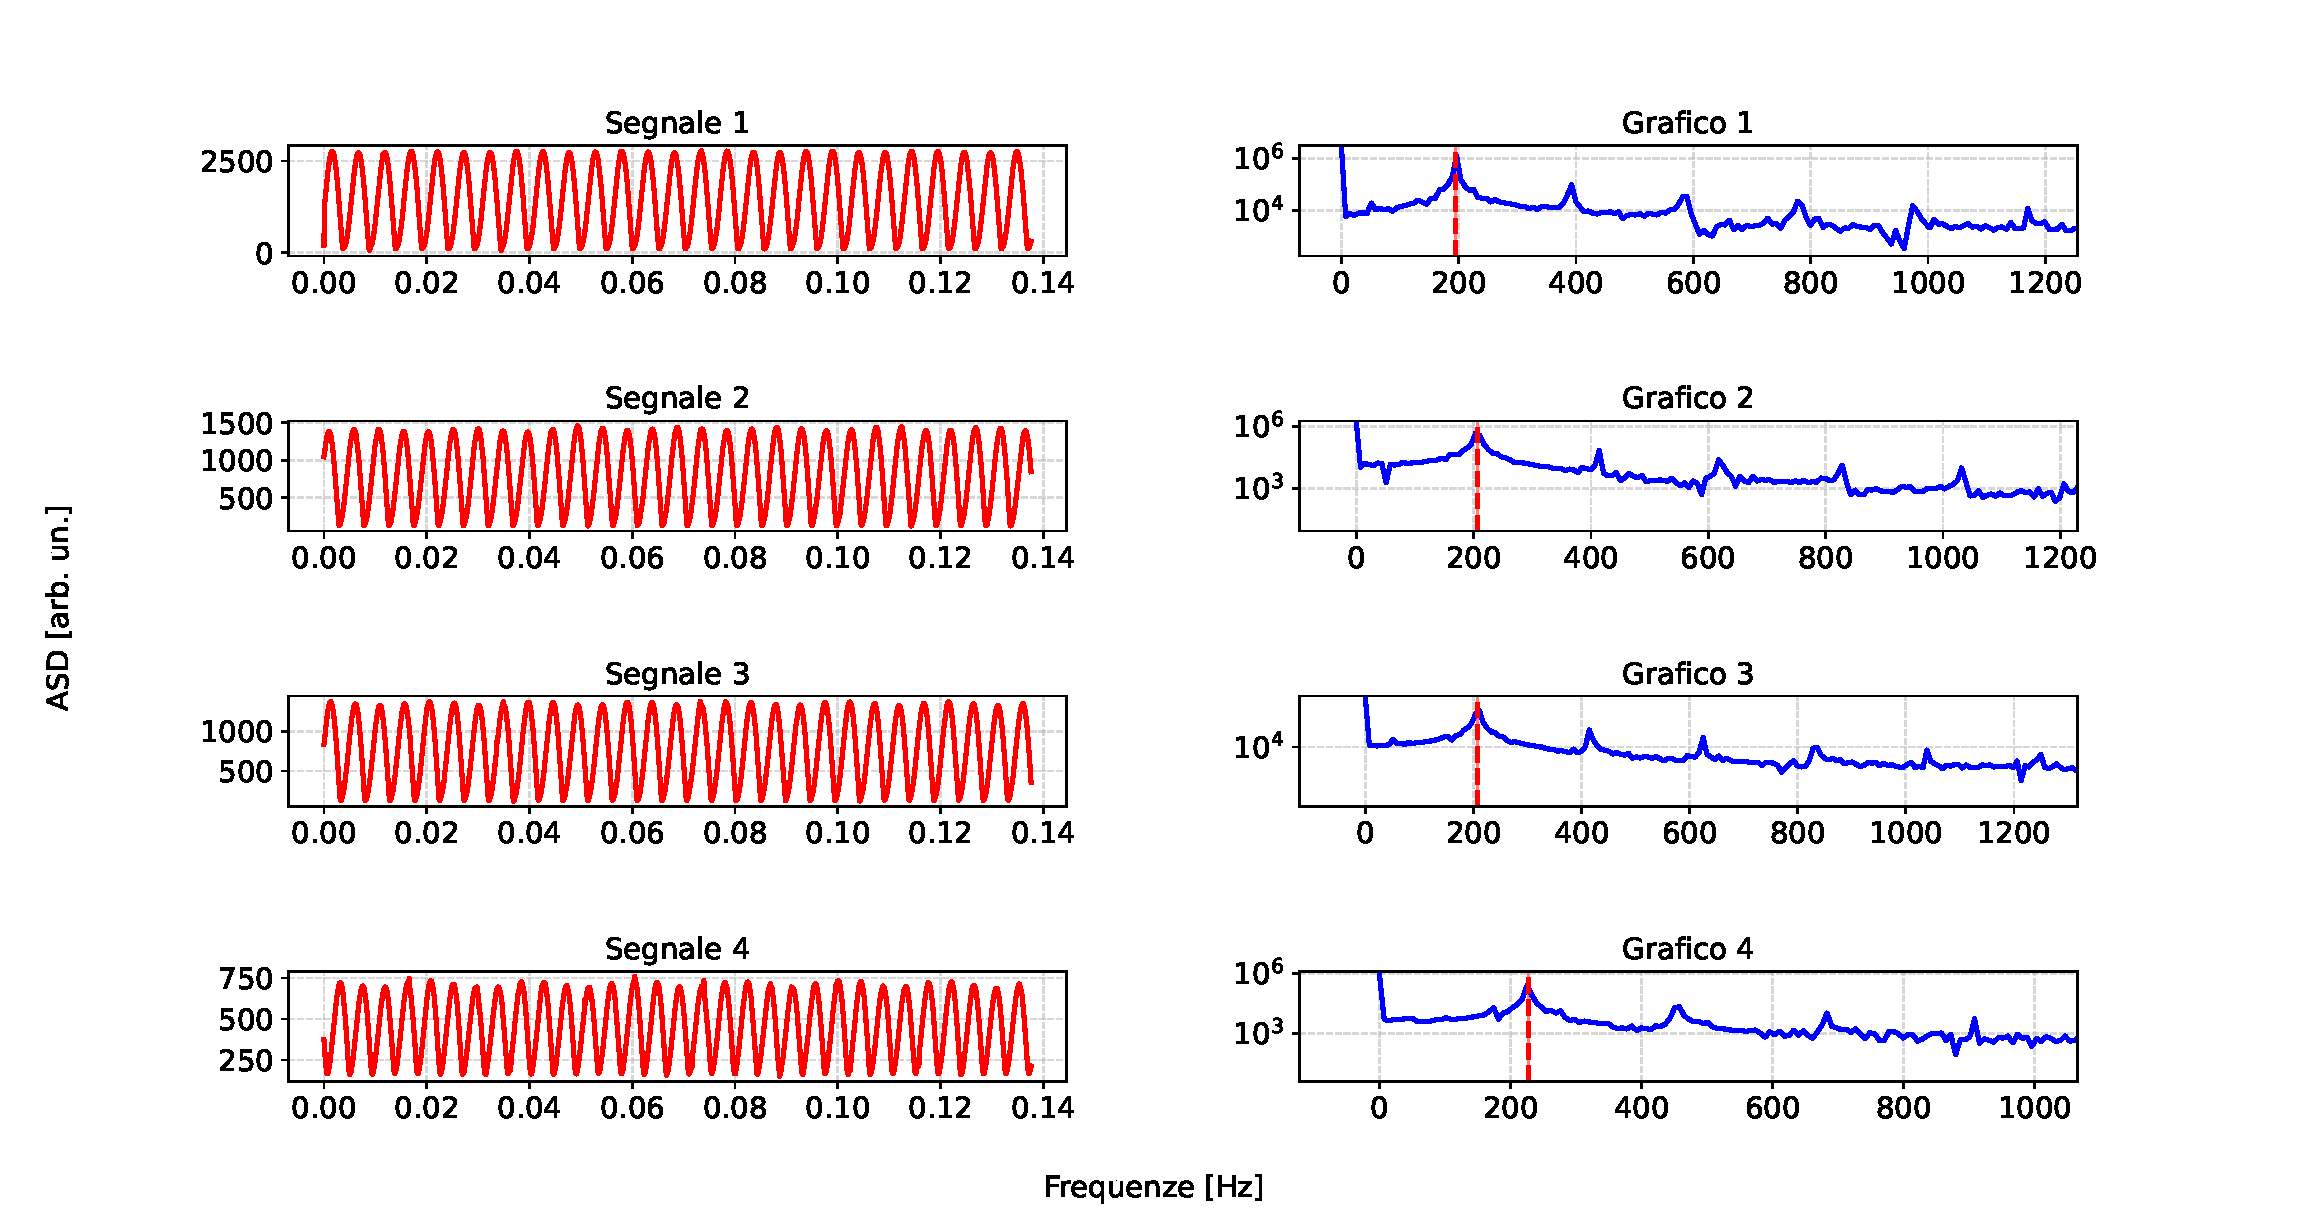
\includegraphics[scale=0.4]{FFT11/first_graph.pdf}
            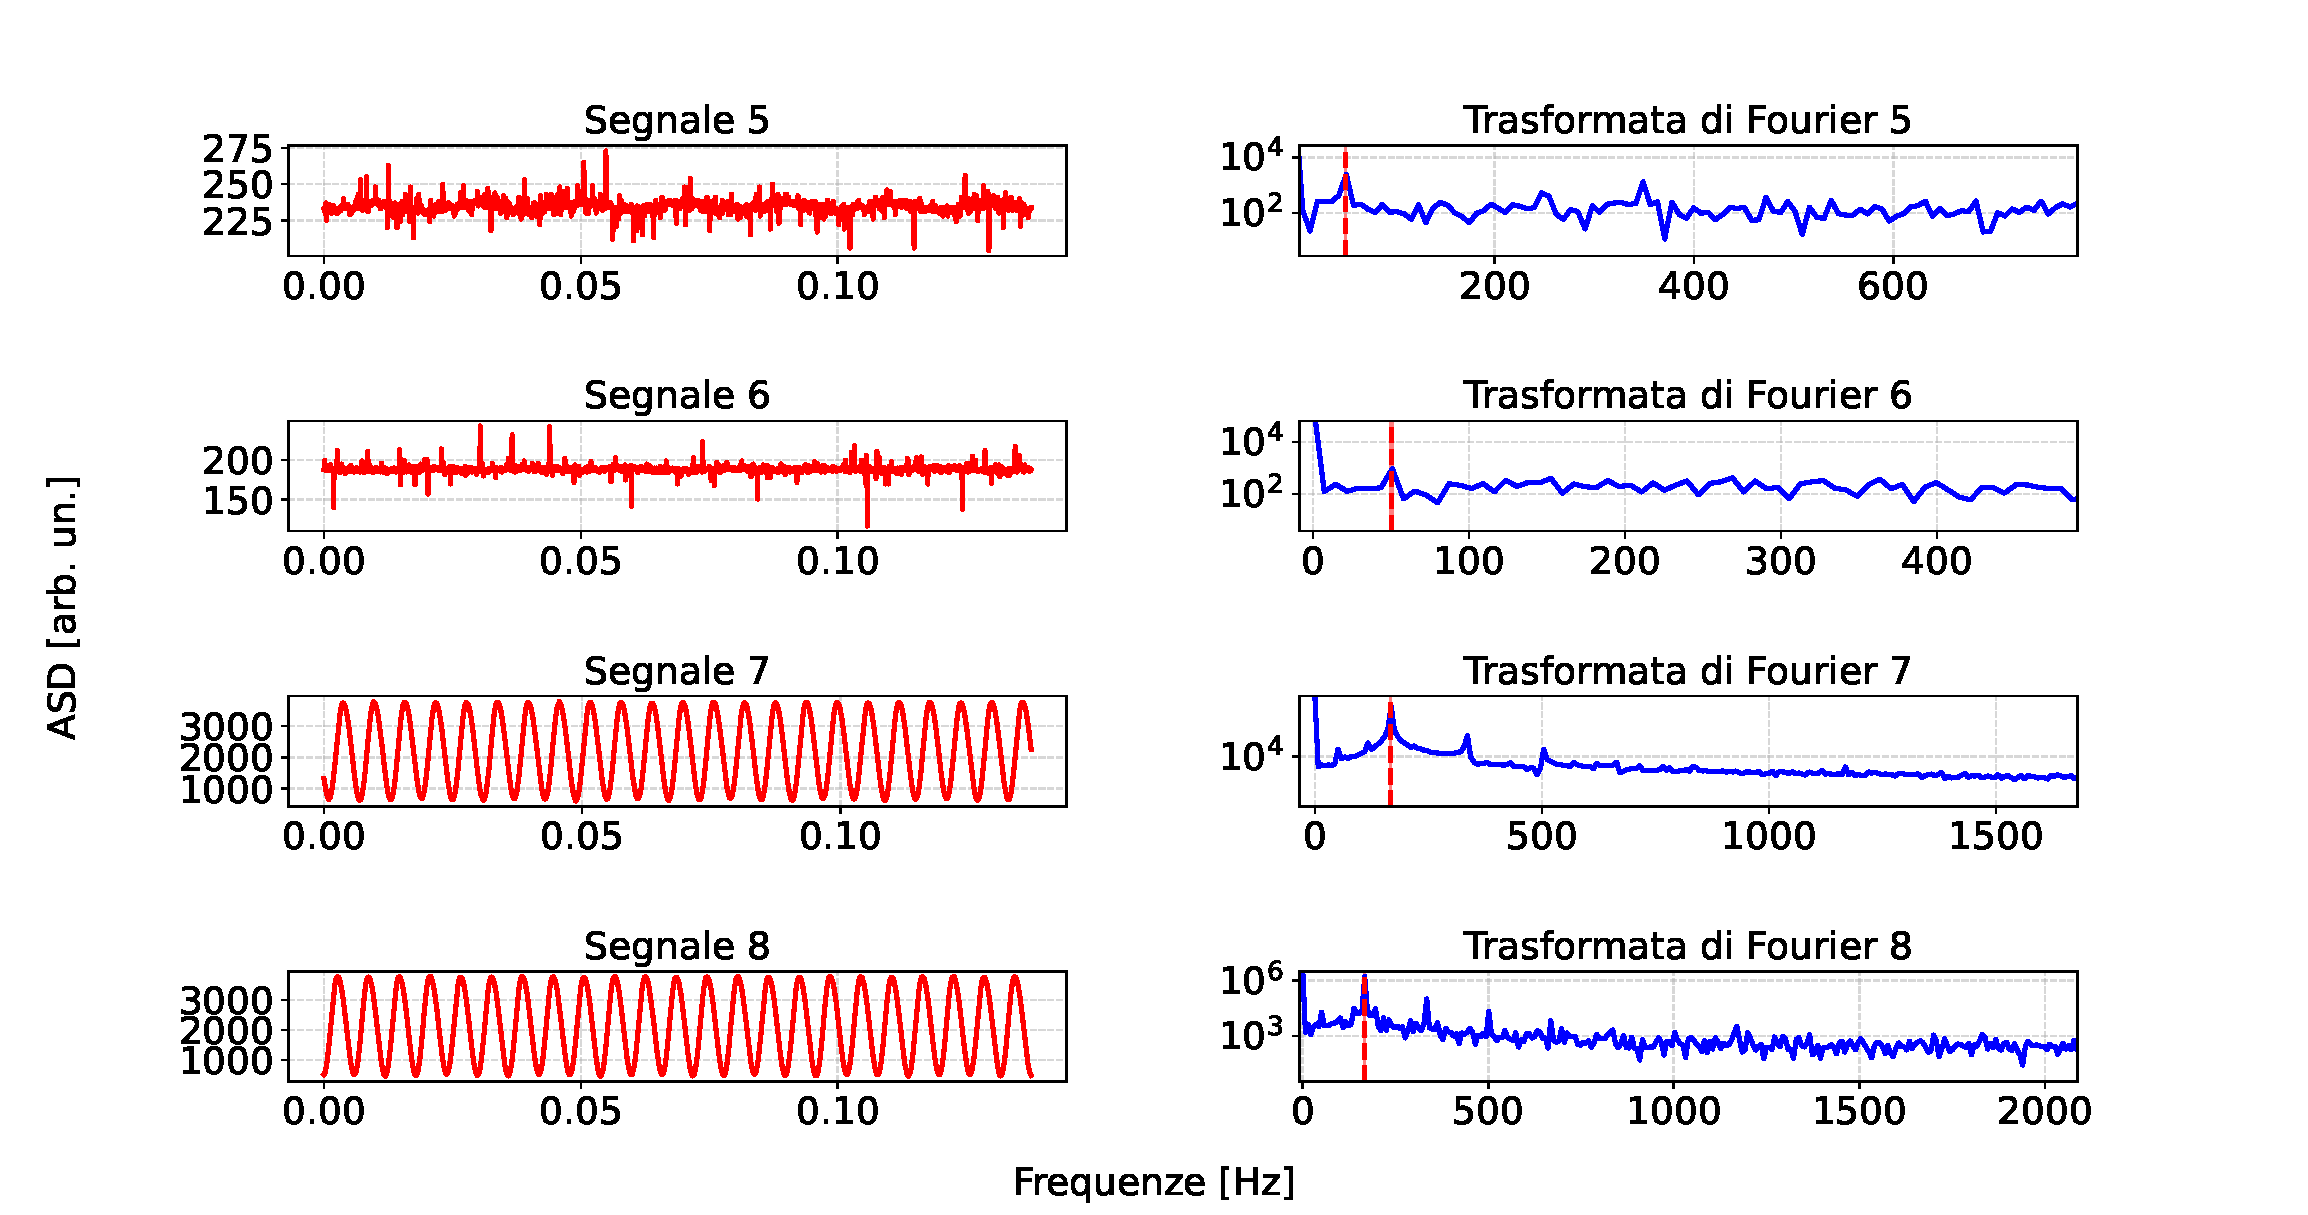
\includegraphics[scale=0.4]{FFT11/second_graph.pdf}
        \end{figure}

        \begin{figure}[H]
            \centering
            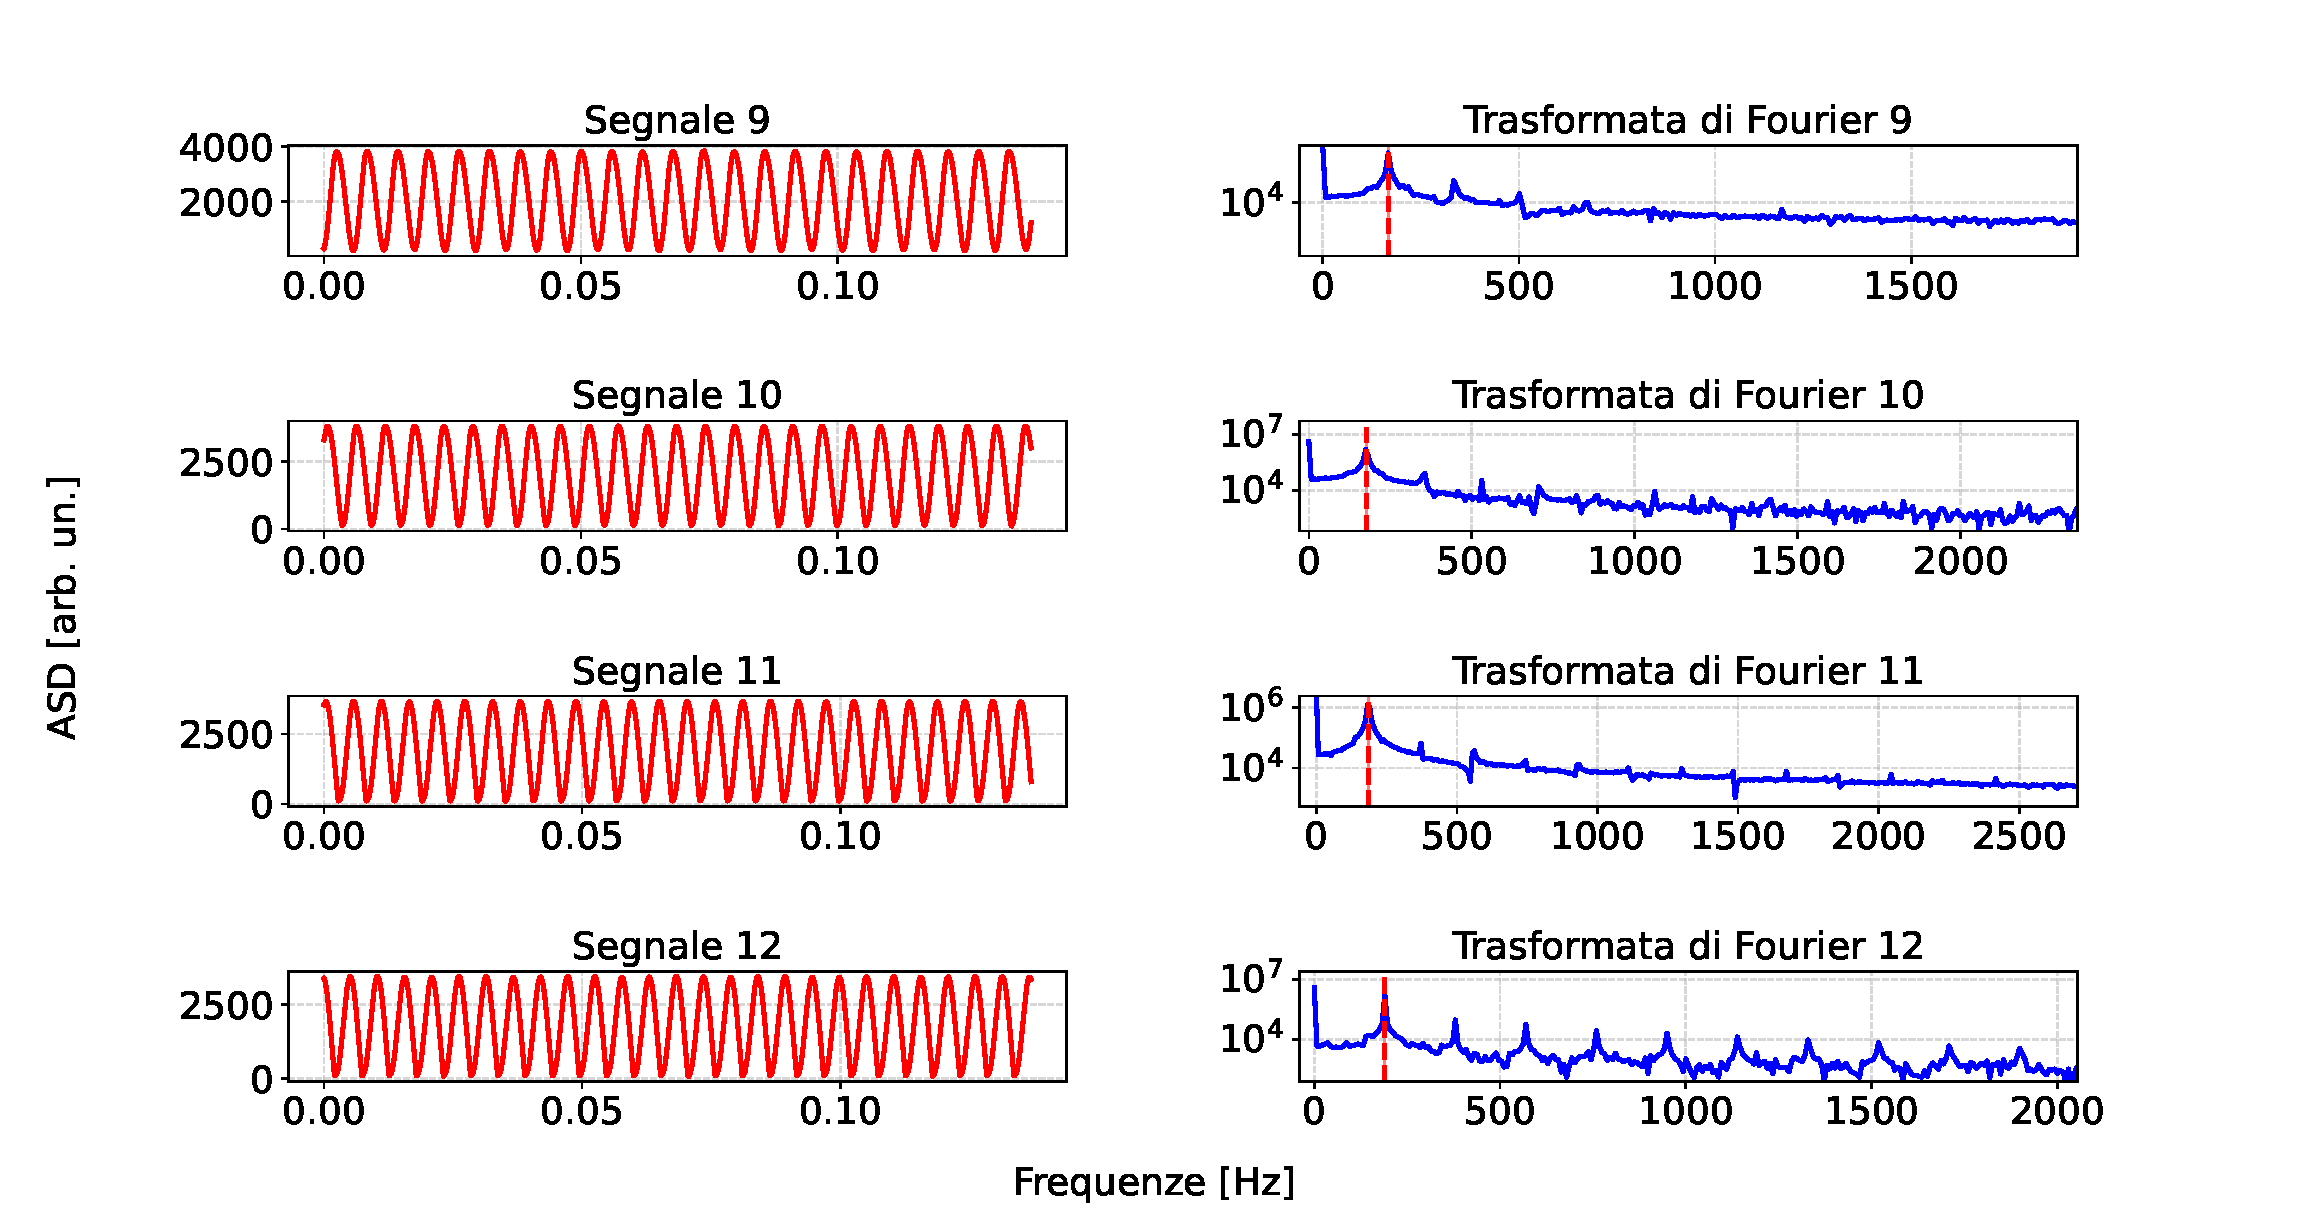
\includegraphics[scale=0.40]{FFT11/third_graph.pdf}
            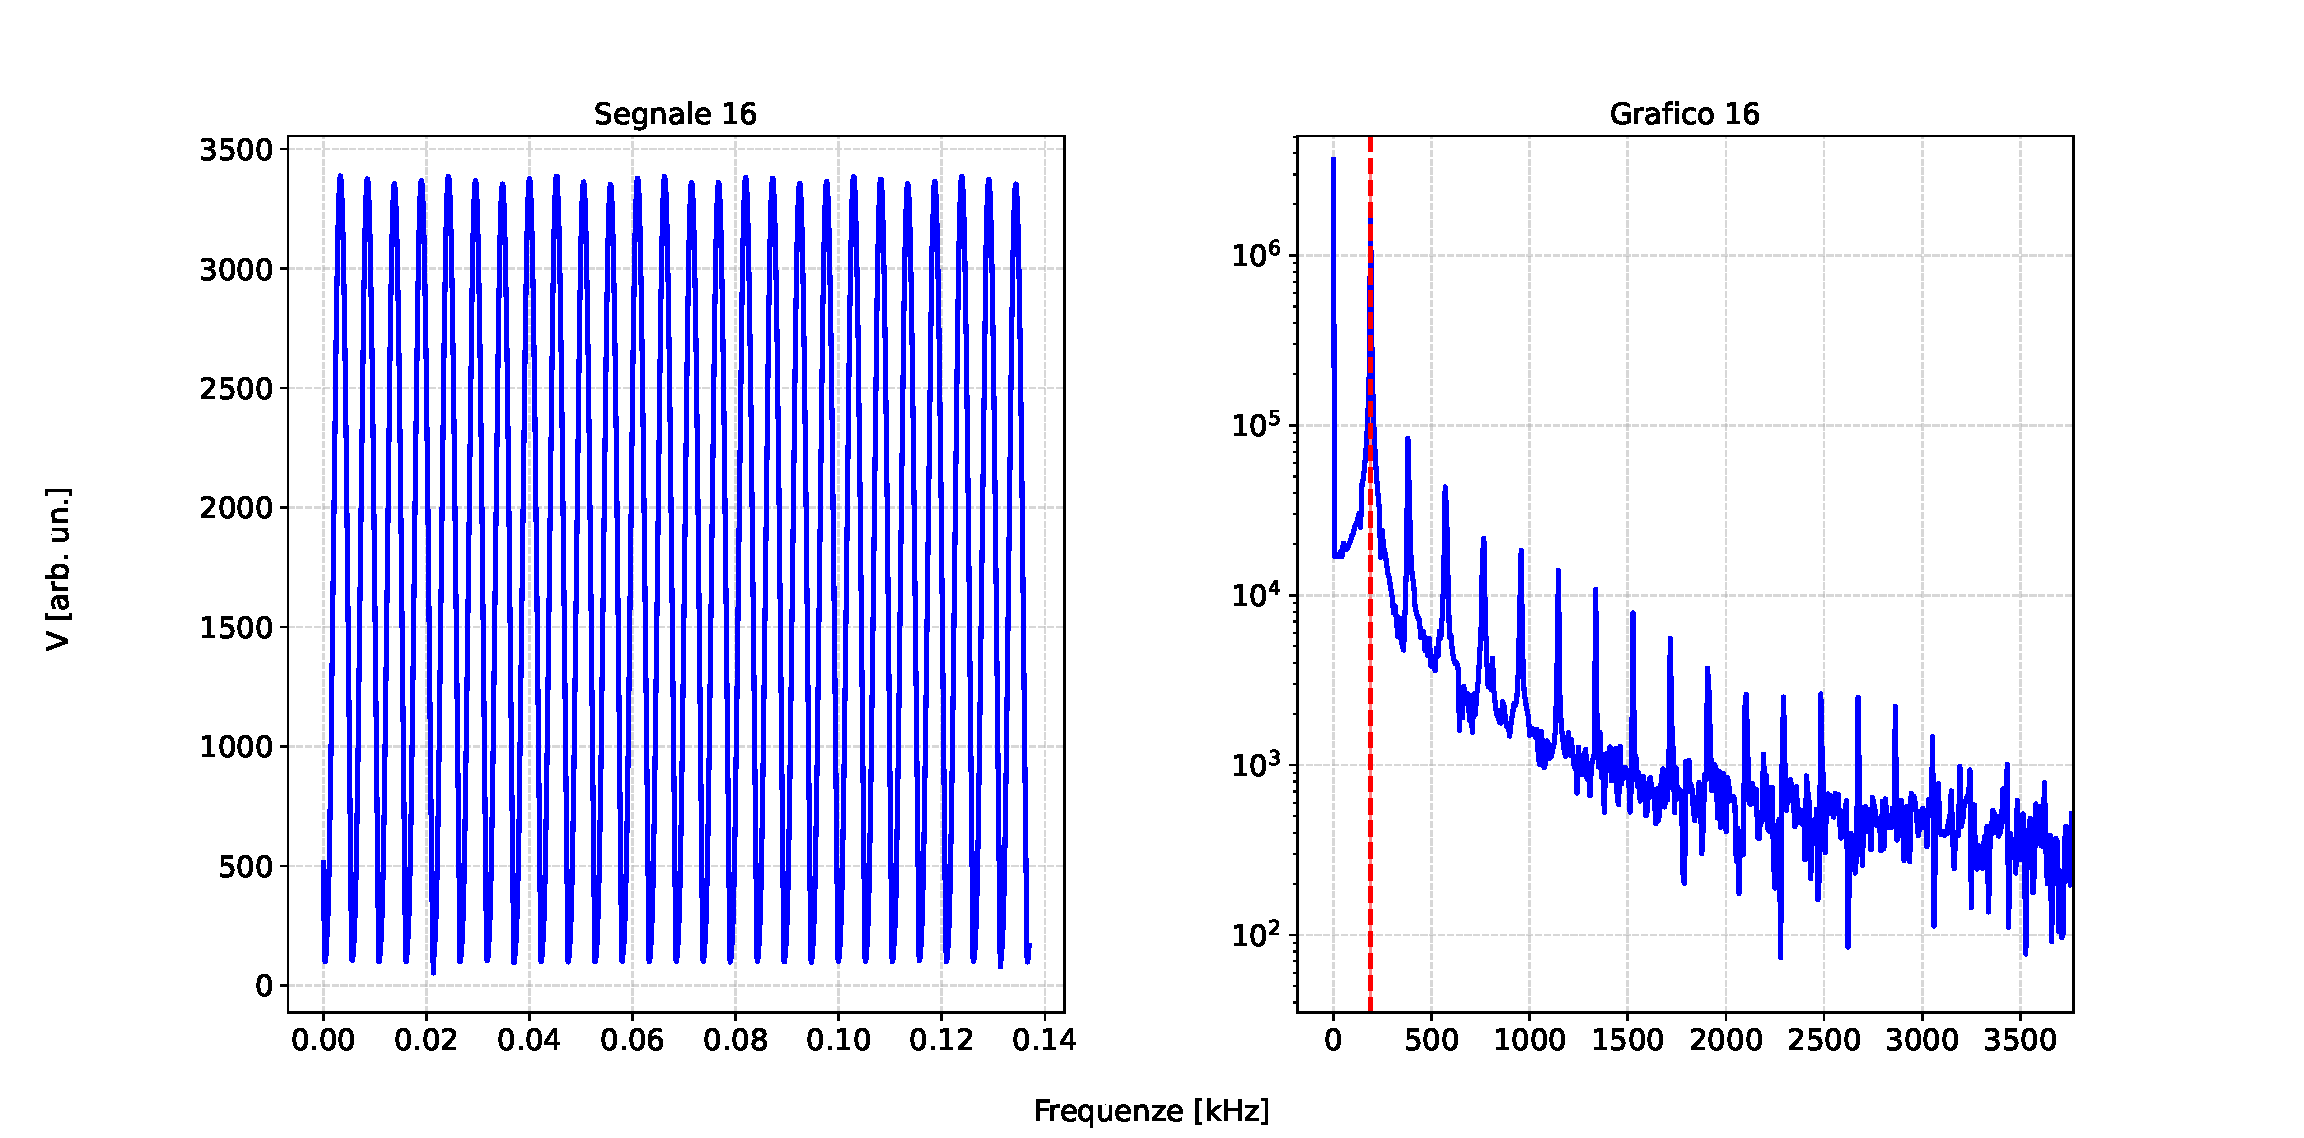
\includegraphics[scale=0.25]{FFT11/fourth_graph.pdf}
            \caption{Segnali con relativa trasformata di Fourier graficata di lato}
            \label{fig:sign_rfft_autoscill}
        \end{figure}

    Prima del confronto con i valori di bestfit, possiamo già osservare che abbiamo un picco a frequenza nulla, coerentemente con quanto atteso. Escludendo quest'ultimo, si nota la presenza di molteplici picchi, quando in realtà ci apettiamo dall'autoscillatore un segnale sinuosodaile "puro" quindi ci aspettiamo due picchi: uno corrispondente alla frequenza nulla e uno corrispondente a quello della frequenza del segnale. Questo è chiaramente dovuto al fatto che non si tratta di un autoscillatore puro e non riesce a produrmi un segnale perfettamente sinusoidale.
    In Tab(\ref{tab:cft_rfft_bestfit}) riportiamo i valori di bestfit

        \begin{table}[H]
            \centering
            \begin{tabular}{c c c}
                \toprule
                $n$ & $f_{0_\text{rfft}} \, [\text{Hz}]$ & $f_{0_\text{bestfit}} \, [\text{Hz}]$ \\
                \midrule
                1 & $195 \pm 7$         & $195.13 \pm 0.06$ \\
                2 & $203 \pm 7$       & $206.61 \pm 0.07$ \\
                3 & $210 \pm 7$         & $207.86 \pm 0.07$ \\
                4 & $225 \pm 7$         & $227.02 \pm 0.08$ \\
                5 & $50 \pm 7$          & $50 \pm 1$ \\
                6 & $50 \pm 7$          & $50 \pm 4$ \\
                7 & $168 \pm 7$         & $167.21 \pm 0.03$ \\
                8 & $167 \pm 7$         & $166.95 \pm 0.03$ \\
                9 & $166 \pm 7$         & $168.10 \pm 0.04$ \\
                10 & $174 \pm 7$        & $176.66 \pm 0.04$ \\
                11 & $182 \pm 7$        & $185.81 \pm 0.03$ \\
                12 & $189 \pm 7$        & $190.06 \pm 0.04$ \\
                13 & $190 \pm 7$        & $190.78 \pm 0.04$ \\
                \bottomrule
            \end{tabular}
            \caption{Tabella con i valori di frequenza del segnale stimata tramite RFFT e tramite bestfit, dove $n$ rappresenta l'$n-$segnale analizzato}
            \label{tab:cft_rfft_bestfit}
        \end{table}
    Si osserva che i valori di frequenza stimati tramite bestfit e tramite RFFT sono compatibili entro le barre di errori per tutti i valori. Come errori sul valore stimato tramite la RFFT si è utilizzata la spaziatura tra un valore della frequenza e quello successivo, che abbiamo scelto, nell'algoritmo della RFFT, di essere pari a 
        $$
            \Delta f = \frac{1}{\max{t}}
        $$
    dove $\max{t}$ è il tempo massimo di acquisizione del segnale.
\section{Oscillazioni smorzate}

        
        \begin{figure}[H]
            \begin{minipage}{0.45\textwidth}
                Sono state prese delle misure di segnale in uscita da un circuito RLC,
                come mostrato in Fig($\ref{fig:osc_diag}$) per tre diversi condensatori.
                Sono stati misurati il periodo e la frequenza delle oscillazioni.
                E' stato eseguito un fit ai minimi quadrati per un'oscillazione 
                smorzata per determinarne il periodo.
                E' stata eseguita una FFT per il medesimo scopo.
                I risultati sono riportati in Tab.($\ref{tab:osc_smor}$) e 
                in Fig.($\ref{fig:osc_smor}$).
            \end{minipage}%
            \hfill
            \begin{minipage}{0.45\textwidth}
                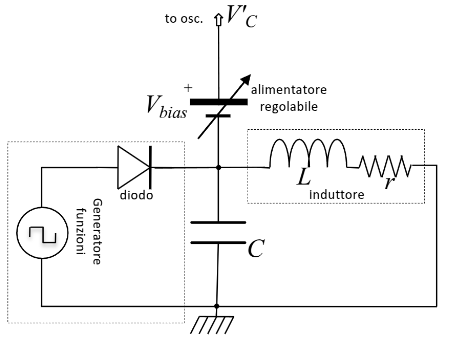
\includegraphics[width=\textwidth]{FFT12/RLCdiagram.png}
                \caption{Diagramma del circuito RLC realizzato.}
                \label{fig:osc_diag}
            \end{minipage}
        \end{figure}

        \begin{figure}[H]
            \centering
            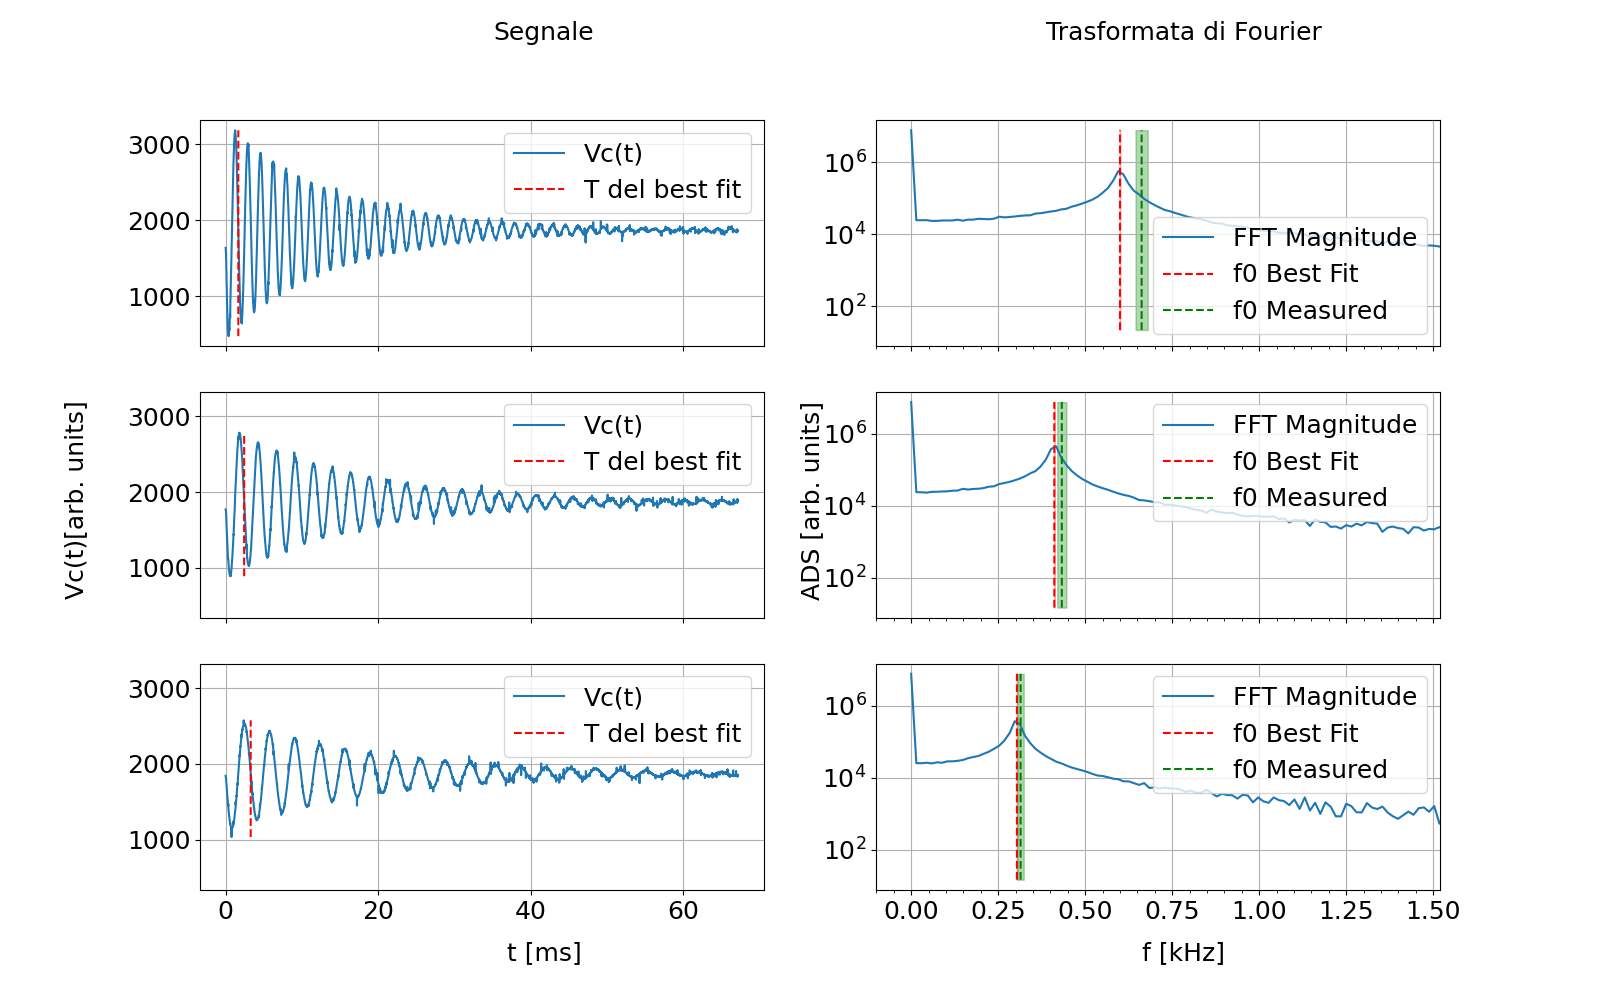
\includegraphics[width=\textwidth]{FFT12/FFTRLC.png}
            \caption{}
            \label{fig:osc_smor}
        \end{figure}

        \begin{table}[H]
            \centering
            \caption{Confronto tra le frequenze di oscillazione misurate con quelle ottenute tramite FFT e bestfit.
                    Attorno ai valori medi è stata rappresentata la barra di errore per il valore
                    misurato e per quello del bestfit, per il quale non si vede essendo molto piccola.}
                \begin{tabular}{cccc}
                    $C$[$\mu$F]          &$f_{0mis}$                &   $f_{0fft}$[kHz]       & $f_{0bestfit}$[kHz] \\
                    \hline
                    $0.1 \pm 20\%tol.$   &     $0.66 \pm 0.02$      & $0.595 \pm 0.004$       & $0.6001 \pm 0.0003$ \\
                    $0.22 \pm 20\%tol.$  &$0.43 \pm 0.01$           & $0.416 \pm 0.004$       & $0.41131\pm 0.00002$ \\
                    $0.47 \pm 20\%tol.$  &$0.314 \pm 0.009 $        &$0.298 \pm 0.004$        & $0.30393\pm 0.00002$ \\
                \end{tabular}
                \label{tab:osc_smor}

        \end{table}
    
    Le frequenze ottenute tramite la FFT e tramite il bestfit sono compatibili, 
    eccetto per la prima frequenza misurata, entro la barra di errore.

    Coerentemente con quanto ci si può aspettare sono presenti 2 picchi nella FFT,
    uno a frequenza nulla, in quanto il segnale non è alternato, l'altro
    alla frequenza di oscillazione del segnale.

    Siccome il segnale non è perfettamente sinusoidale, la FFT
    presenta un ampio spettro di armoniche attorno al picco principale.

\section{Materiali nel core dell'induttore}
\begin{figure}[H]
    \begin{minipage}{0.45\textwidth}
        Sono state prese delle misure di segnale in uscita da un circuito RLC,
        come mostrato in Fig($\ref{fig:mat_diag}$) inserendo diversi materiali dentro 
        il core dell'induttore.
        E' stato eseguito un fit ai minimi quadrati per un'oscillazione 
        smorzata per determinarne il periodo e il tempo di smorzamento.
        E' stata eseguita una FFT per determinare il periodo di oscillazione.
        I risultati sono riportati in Tab.($\ref{tab:mat_smor}$) e 
        in Fig.($\ref{fig:mat_smor}$).
    \end{minipage}
    \hfill
    \begin{minipage}{0.45\textwidth}
        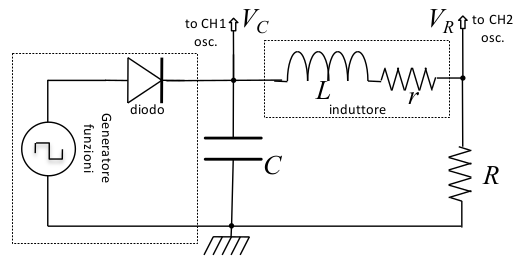
\includegraphics[width=\textwidth]{FFT13/RLCmaterialsdiagram.png}
        \caption{Diagramma del circuito RLC realizzato.}
        \label{fig:mat_diag}
    \end{minipage}
\end{figure}

        \begin{figure}[H]
            \centering
            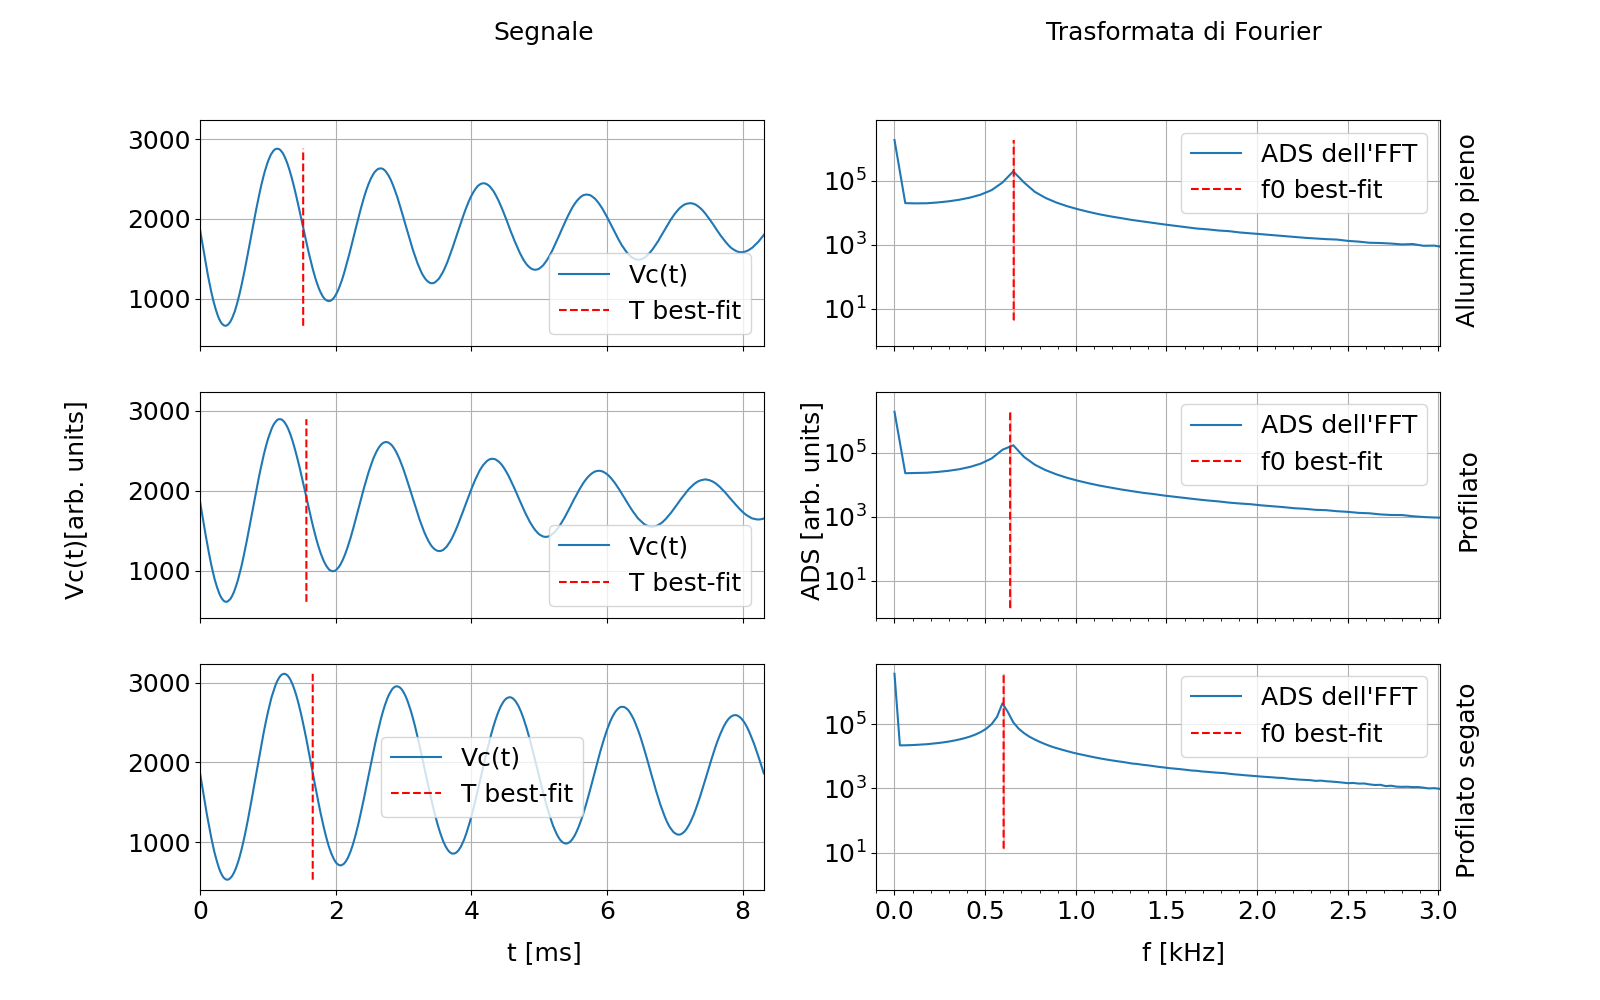
\includegraphics[width=\textwidth]{FFT13/FFTMATERIALS1.png}
            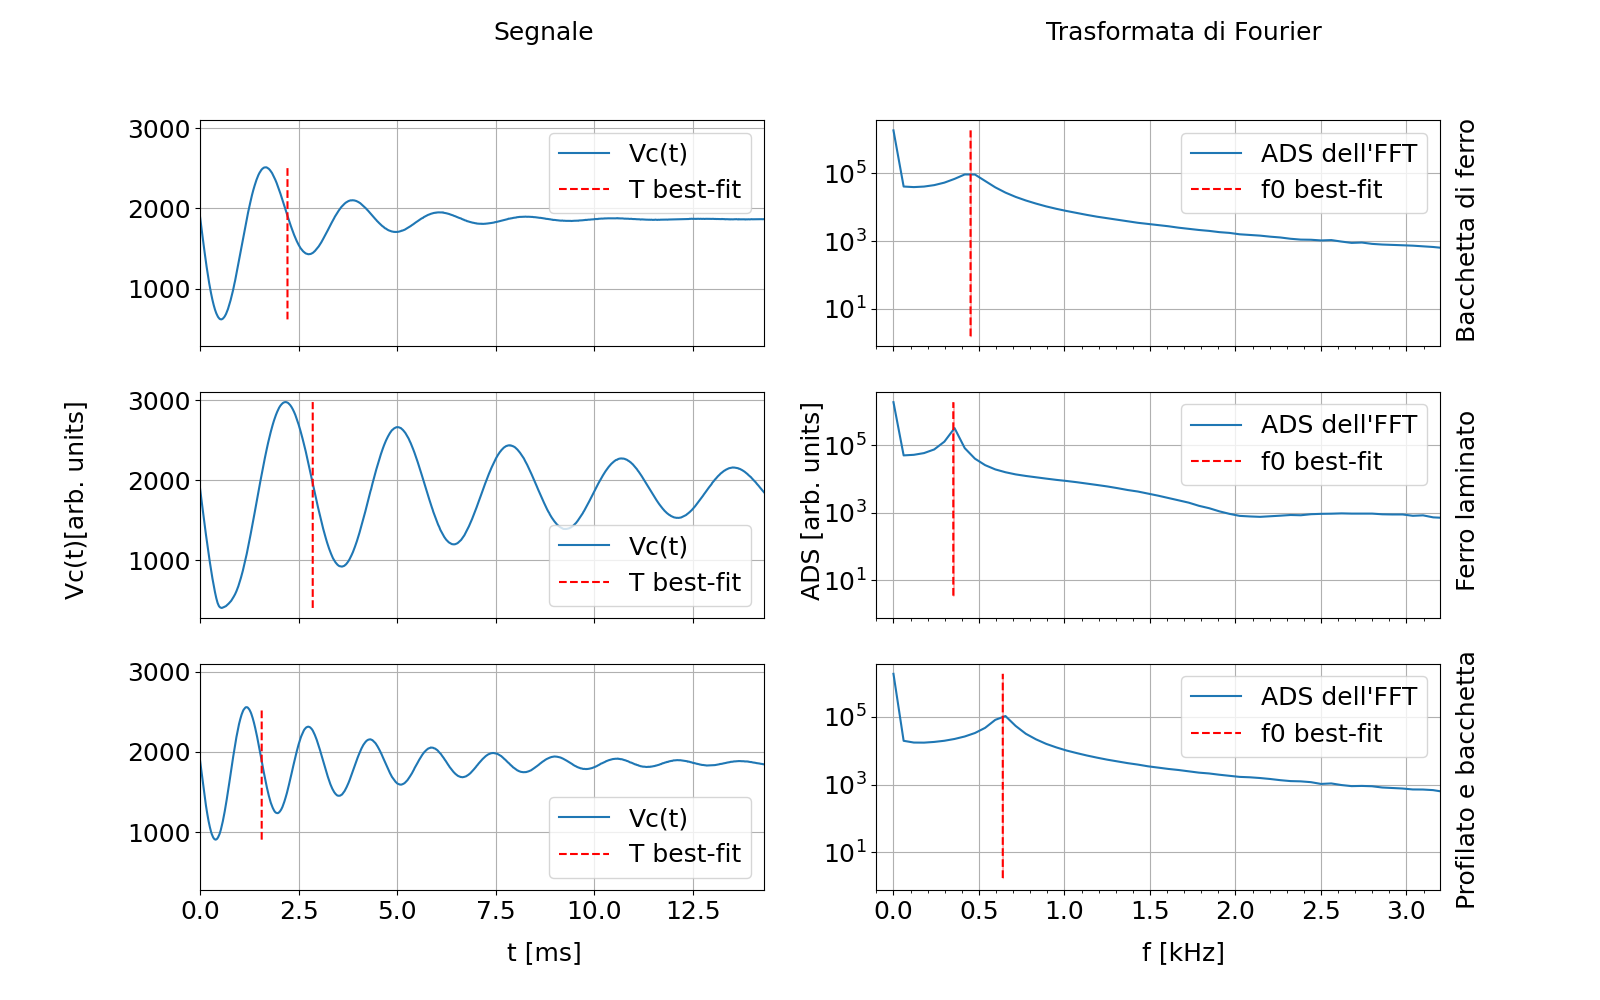
\includegraphics[width=\textwidth]{FFT13/FFTMATERIALS2.png}
            \caption{Confronto tra le frequenze di oscillazione misurate con quelle ottenute tramite FFT e bestfit.
            Attorno ai valori medi è stata rappresentata la barra di errore per il valore
            misurato e per quello del bestfit, per il quale non si vede essendo molto piccola.}
            \label{fig:mat_smor}
        \end{figure}

        \begin{table}[H]
            \centering
            \caption{Confronto tra le frequenze di oscillazione misurate con quelle ottenute tramite FFT e bestfit.
                    Attorno ai valori medi è stata rappresentata la barra di errore per il valore
                    misurato e per quello del bestfit, per il quale non si vede essendo molto piccola.}
                \begin{tabular}{ccc}
                    materiale           &   $f_{0fft}$[kHz]     & $f_{0bestfit}$[kHz] \\
                    \hline
                    Alluminio pieno     & $0.65\pm0.02$         & $0.657\pm0.008$ \\
                    Profilato           & $0.65\pm0.02$         & $0.637\pm0.008$ \\
                    Profilato segato    & $0.595\pm0.009$       & $0.601\pm0.002$ \\
                    Bacchetta di ferro  & $0.42\pm0.02$         & $0.451\pm0.009$ \\
                    Ferro laminato      & $0.35\pm0.02$         & $0.349\pm0.009$ \\
                    Profilato e bacchetta& $0.65\pm0.02$        & $0.639\pm0.009$ \\  
                \end{tabular}
                \label{tab:mat_smor}

        \end{table}

        Le frequenze ottenute tramite la FFT e tramite il bestfit sono compatibili, 
        eccetto per la bacchetta di ferro, entro la barra di errore.
        Il problema con la bacchetta di ferro è che essendo il segnale molto smorzato 
        e il picco non è molto pronunciato; in aggiunta siccome l'acquisizione non è stato
        possibile prenderla suffiecienemente lunga -in quanto il segnale sarebbe stato 
        eccessivamente soppresso-, si sovrappone al problema precedente 
        uno legato alla scarsa risoluzione dei punti nello spettro delle frequenze.

        
        Si può osservare che per i blocchi di alluminio pieno e profilato di alluminio,
        il periodo di oscillazione diminuisce, in quanto è diamagnetico e il periodo
        è inversamente proporzionale all'induttanza,che diminuisce.
        
        Analogamente per il ferro laminato e ,in maggior misura, per la bacchetta di 
        ferro il periodo di oscillazione aumenta per il comportamento da ferromagnete.
        
        Nella discussione appena fatta sto trascurando il contributo dato dal 
        tempo caratterstico di smorzamento al periodo di oscillazione.
        
        Il tempo caratteristico di smorzamento è rilevante nei grafici 
        delle FFT, Fig($\ref{fig:mat_smor}$), in quanto impone l'ampiezza del picco:
        si osserva che questo aumenta per ogni materiale inserito nel core 
        rispetto a quanto visto nel caso  del vuoto visto a Fig.($\ref{fig:osc_smor}$).
        Tuttavia questo non accade per il profilato segato dove, è possibile  
        aspettarsi che gli effetti delle correnti parassite siano meno importanti.

        





\section{"Il pinnacolone"}

\section{Glicemia}

        E' stata acquisita la Glicemia di un paziente di diabete mellito tipo 1 in 
        due periodi diversi: le vacanze natalizie e la sessione di studio per gli esami.
        I risultati dell'analisi con FFT sono riportati in Fig.($\ref{fig:rubbish}$).
        I due periodi sono paragonabili in quanto ravvicinati e si assume che
        la temperatura e lo stess non abbiano subito variazioni significative 
        nel paziente.
        
        Si evidenziano i tempi che determinano le frequenze caratteristiche dell'andamento glicemico:
            \begin{itemize}
                \item 3 ore - il tempo di effetto dell'insulina
                \item 6 ore - il tempo che durante il giorno intercorre tra i parassite
                \item 24 ore - il giorno (da cui il sonno, la produzione ormonale, le attività
                svolte...)
            \end{itemize}
            \begin{figure}[H]
                \centering
                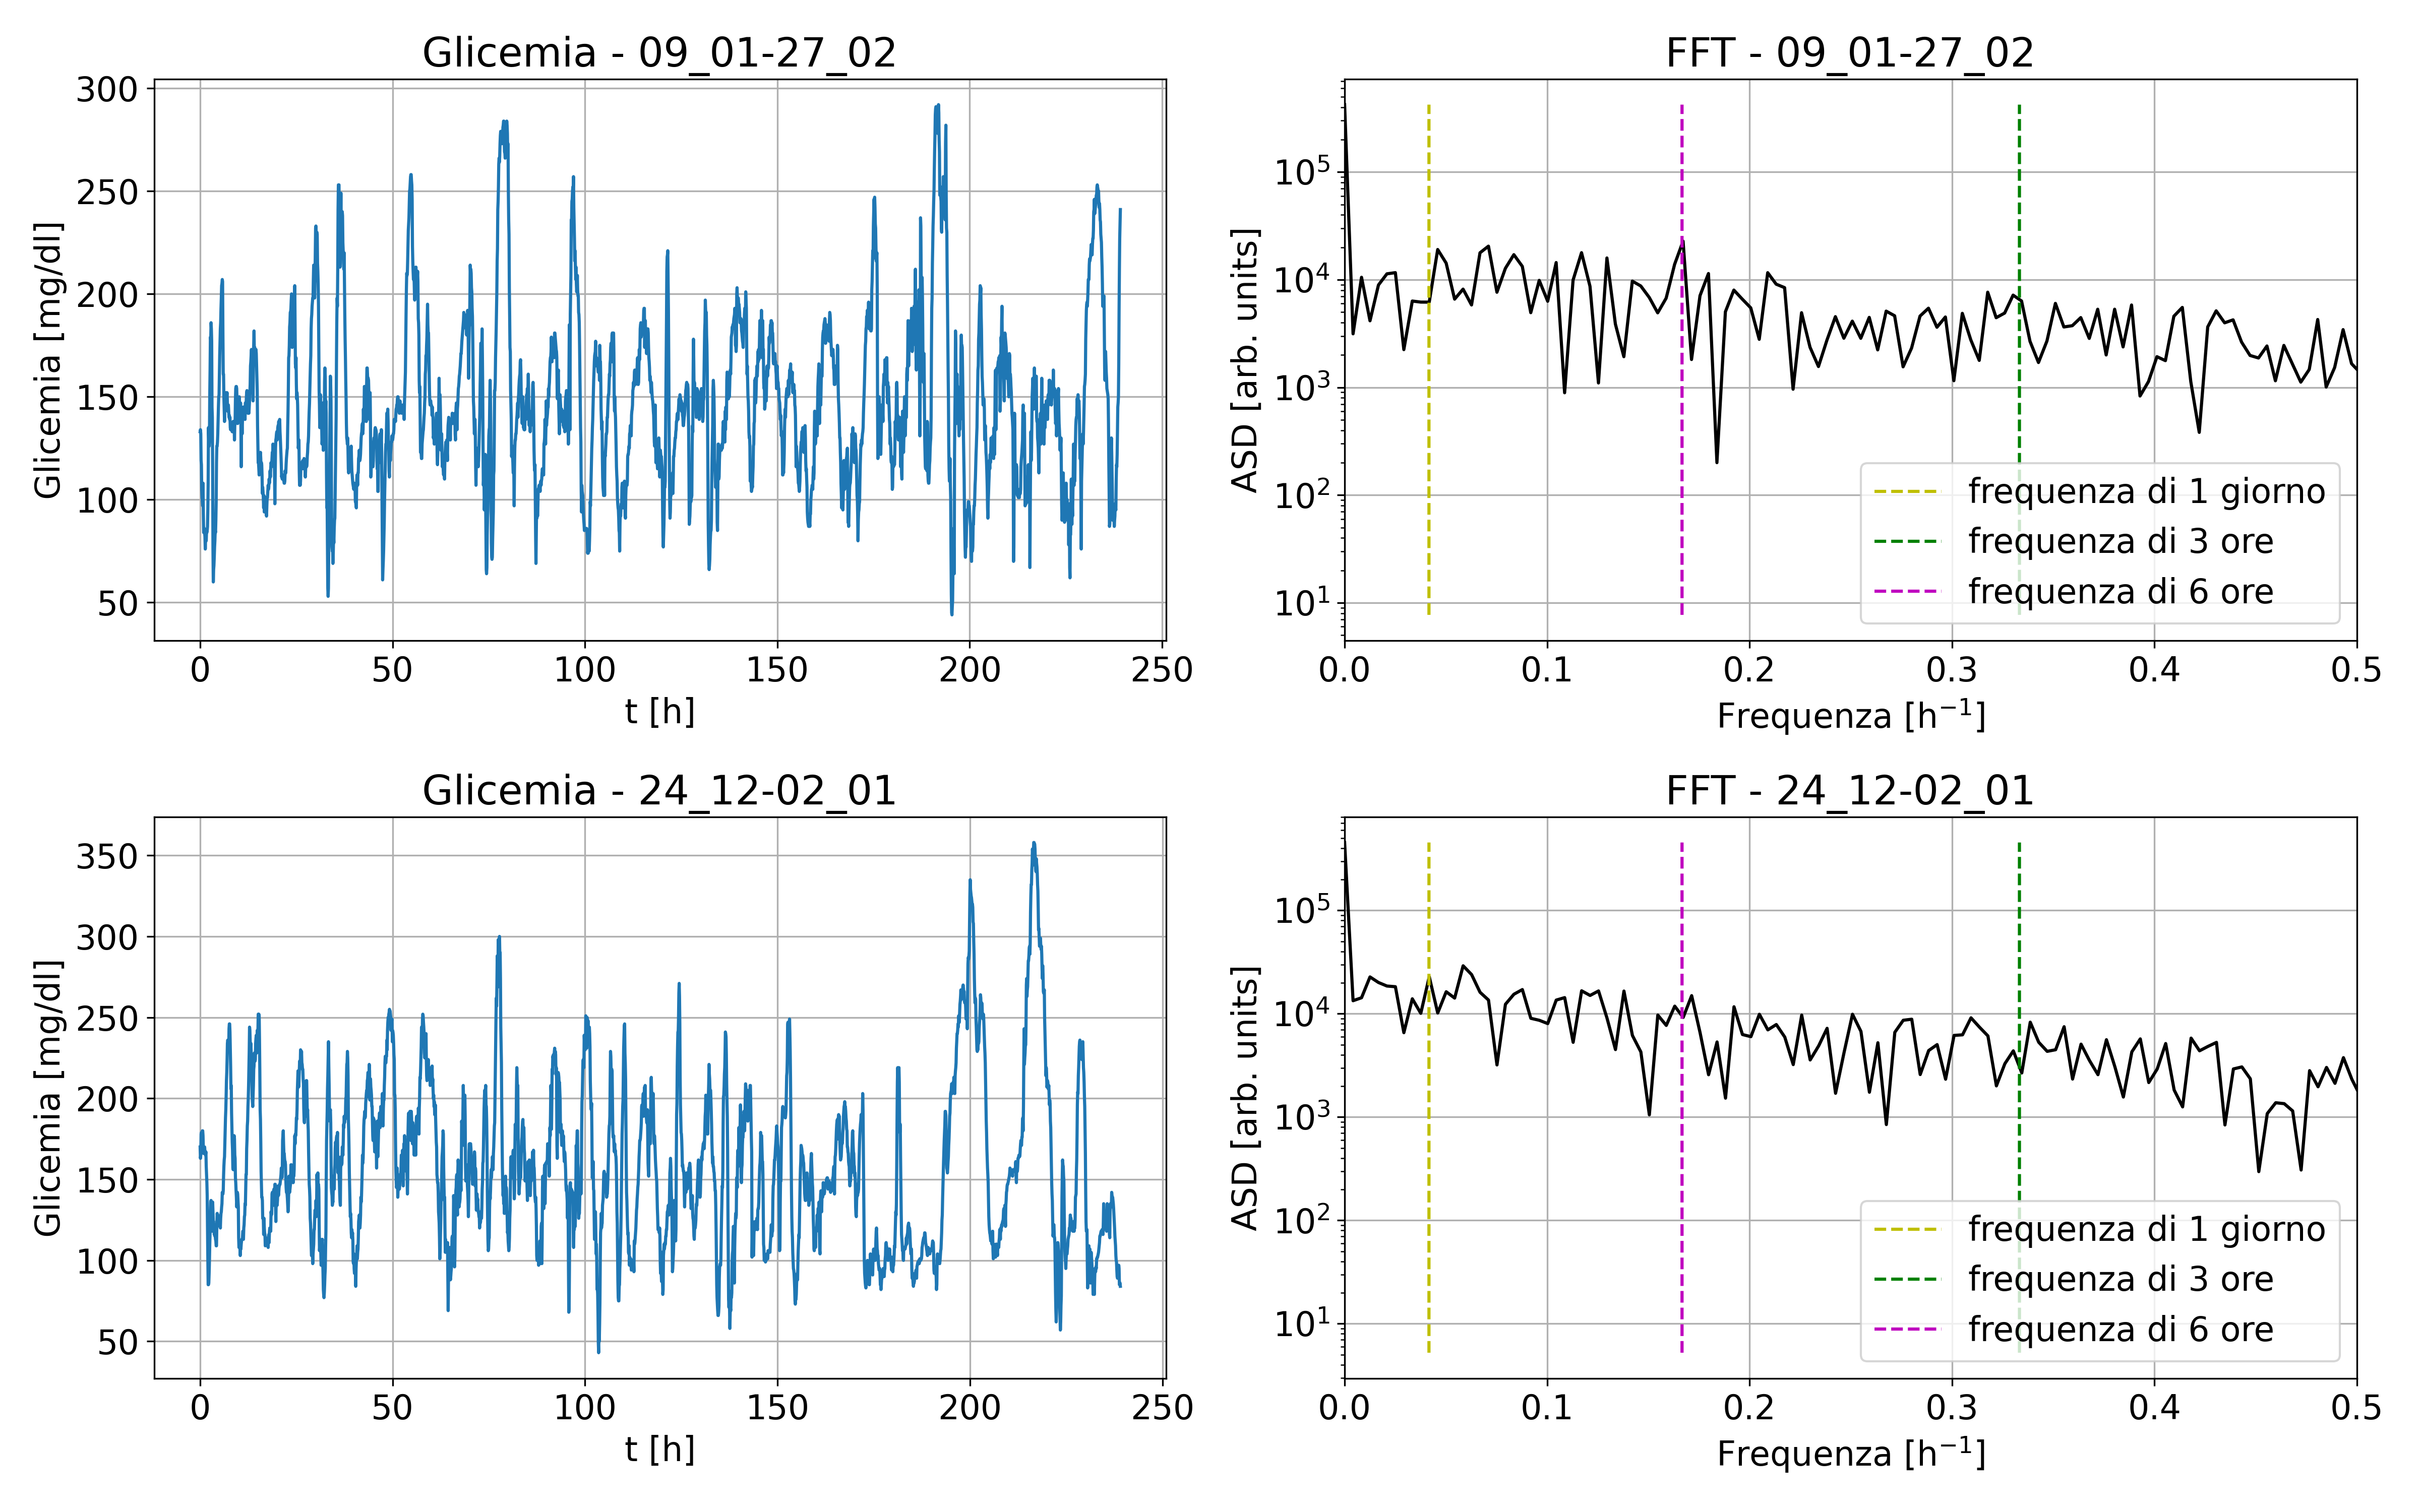
\includegraphics[width=\textwidth]{rubbish/rubbish.png}
                \caption{E' evidente la presenza di una maggiore regolarità nel 
                periodo di studio rispetto alle festività: il picco legato
                al giorno e quello legato ai scompare durante le festività 
                per le persistenti iperglicemie dovute all'aumentata insulino-resistenza e ai pasti più ricchi di grassi.
                Il picco legato all'azione dell'insulina si attenua probabilmente
                a causa dell'elevata insulino-resistenza.}
                \label{fig:rubbish}
            \end{figure} 

\end{document}